\documentclass[main.tex]{subfiles}
\begin{document}
\subsection{高分子无热溶液}
\begin{wrapfigure}{r}{0.333\textwidth}
  \centering
  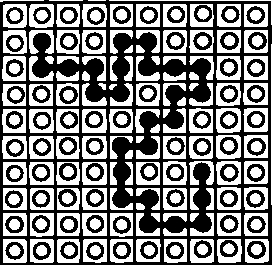
\includegraphics[width=\linewidth]{../images/lattice_flory_huggins.pdf}
  \caption{一条高分子链的链段在网格中的一种放置方式。}
  \label{fig:lattice_flory_huggins}
\end{wrapfigure}

在前面几节,我们考虑的情况是溶质和溶剂分子大小相当,都占1个格子。在这种情况下,只要混合焓变为零,任一格子既可以放溶剂分子,也可以放溶质分子,溶液的构形数就是简单的二项式系数
\[\left(\begin{array}{cc}N\\N_1\end{array}\right)=\frac{N!}{N_1!N_2!}\]
由此我们得出了理想溶液的混合熵变。如果溶质分子比溶剂分子大,在格子模型中的效果是溶质分子占据多个格子,那么就算不考虑混合焓变,溶液构形数的计数也不会是简单的二项式系数,可以预见这将导致混合熵变的表达式偏离理想溶液的形式。也就是说,分子尺寸不同的组成,就算混合焓为零,也不是理想溶液。我们将这种情况称为\emph{无热溶液(athermal solution)}。“无热”是指$\Delta_\text{mix}H=0$,但仅此而已。一般地无热溶液的混合熵$\Delta_\text{mix}S\neq\Delta_\text{mix}S^\text{id}$,也就是其超额混合熵$\Delta_\text{mix}S^\text{E}\neq 0$。

如图\ref{fig:lattice_flory_huggins}所示,考虑$N_1$个溶剂分子和$N_2$个聚合度为$r$的高分子,总格子数$N=N_1+rN_2$。这里我们把高分子视为占据$r$个相连格子的大分子,每个格子放置的称为高分子的一个“链段”。这里所谓“链段”仅具有格子模型下的意义,跟高分子物理中其他理论中的“链段”(例如库恩链段)没有直接的关系。

仍记网格的配位数为$z$,则每个溶剂分子周围有$z$个相邻的分子或链段,但每个高分子周围相邻的格子数则不是$rz$,而是要比这个数少。我们先假定高分子是线形长链,那么它将有两个链端链段,每个有$z-1$个相邻的格子;同时有$r-2$个中间链段,每个中间链段周围有$z-2$个相邻格子。因此整个高分子周围的相邻格子数将是
\[qz=2\left(z-1\right)+\left(r-2\right)\left(z-2\right)=rz-2r+2\]
这里引入了参数$q$来表示上面的式子,仅为了后续结果形式简洁。

注意到,这个式子也适用于支化的高分子。在一个支化高分子中,一个支化点链段,将比线形高分子的中间链段少$f-2$个相邻格子($f$是这个支化点的官能度),但由于这个支化点的存在,整个高分子又会比线形高分子多$f-2$个链端,每个链端的相邻格子数是比线形高分子的中间链端多1个的,所以总是能扯平维持上式。

若记高分子的链段是P,溶剂分子是S,$f\left(\text{S}\right)$是任一格子被溶剂占据的概率,$f\left(\text{P}\right)$是任一格子被链段占据的概率,那么在平衡态下,我们有
\[f\left(\text{S}\right)=\phi_1,\quad f\left(\text{P}\right)=\phi_2\]
其中
\[\phi_1\equiv\frac{N_1}{N_1+rN_2},\quad\phi_2\equiv\frac{rN_2}{N_1+rN_2}\]
是溶剂和溶质的体积分数(已假定每个格子的体积相等)。但是,这个简单的练习并不直接得到溶液的构形数。以下我们按照E. Guggenheim的办法\cite{Guggenheim1952,Tompa1956},不用直接计数构形数,可以直接得到高分子溶液的混合熵。这个办法的步骤比较长,以下分成了3个步骤来介绍。

第一步,我们考虑溶液中第一格为X、同时相邻的第二格为Y的概率(X、Y代表S或P)$f\left(\text{XY}\right)$。在这里PP不是同一条链的两个键接链段——后面这种情况我们用$\overline{\text{PP}}$来表示。我们需要写出概率$f\left(\text{SS}\right)$、$f\left(\text{SP}\right)$、$f\left(\overline{\text{PP}}\right)$和$f\left(\text{PP}\right)$。

我们把首个放置的位置视为“中心”位置。它的相邻格子视为这个中心位置所“生出”的。每个溶剂分子中心将生出$z$个相邻位置,而每个高分子总共生出$qz$个相邻位置。如果我们把溶液中的每个分子作为中心都看一遍,它们生出的相邻位置数全加起来,这个总数将是$\left(N_1+qN_2\right)z$。它当然是超过网格本身的格子总数$N$的。我们把这个$\left(N_1+qN_2\right)z$总数解读为溶液中所有“有序相邻对”的个数。用“有序”一词是因为我们区分了一对格子中谁是“中心”谁是“生成”,因此无序对SS将会分别以第一个S为中心($\text{S}\rightarrow\text{S}$和第二个S为中心($\text{S}\leftarrow\text{S}$)的方式被计算两次。我们这里需要计算的概率是有序相邻对的概率。在下一节讨论混合焓变时,我们将考虑无序对的概率。

我们先讨论$f\left(\text{SS}\right)$和$f\left(\text{SP}\right)$已知任一格子是溶剂分子的概率是$f\left(\text{S}\right)=\phi_1$。给定一个放了溶剂的格子,它生出的相邻位置放置了溶剂的概率,在平衡态下,应是所有有序相邻对中$\text{S}\rightarrow\text{S}$的个数比上总有序相邻对个数的比值,即
\[\xi_1\equiv\frac{N_1 z}{\left(N_1+qN_2\right)z}=\frac{N_1}{N_1+qN_2}\]
因此
\[f\left(\text{SS}\right)=\phi_1\xi_1\]
类似的推理有
\[f\left(\text{SP}\right)=\phi_1\xi_2,\quad \xi_2\equiv\frac{qN_2}{N_1+qN_2}\]

我们再来考虑$f\left(\text{PS}\right)$、$f\left(\text{PP}\right)$和$f\left(\overline{\text{PP}}\right)$。给定一个位置被P占据的事实下,它周围相邻位置有多少可放置其他链段P(除开与自身键接的$\overline{P}$之外)以及溶剂分子S的空格呢?这似乎还要取决于这个$P$是一个链端、一个中间链段、还是一个支化点链段。但我们用整个高分子的平均结果来讨论。如果不是因为高分子链段的连接性,每个高分子($r$聚体)周围应有$rz$个相邻格子可以放链段和溶剂分子。现在由于高分子的连接性,每个高分子只生出$qz$个相邻格子,以供放置P和S。因此,平均而言一个高分子链段周围的$z$个格子中的任一个,放置了P或S的比例或概率是$q/r$,放置了$\overline{P}$的概率就是$1-q/r$。因此
\[f\left(\text{PS}\right)=\phi_2\frac{q}{r}\xi_1,\quad f\left(\text{PP}\right)=\phi_2\frac{q}{r}\xi_2\]
于是
\[f\left(\text{PS}\right)+f\left(\text{PP}\right)=\phi_2\frac{q}{r}\]
就是给定一个格子是链段,其相邻的格子不是$\overline{\text{P}}$的概率。这里用到了$\xi_1+\xi_2\equiv 1$。易得
\[f\left(\overline{\text{PP}}\right)=1-\left[f\left(\text{PS}\right)+f\left(\text{PP}\right)\right]=\frac{r-q}{r}\phi_2\]

推广至连续$r$个格子的情况。不难得出,$f\left(\text{SSS}\right)=\phi_1\xi_1^2,\cdots,f\left(r\text{S}\right)=\phi_1\xi_1^{r-1}$。$f\left(\overline{r\text{P}}\right)$并不能简单推广出明显的表达式,但可以保证的是至少它正比于$\phi_2$,因此可记$f\left(\overline{r\text{P}}\right)=K^\prime\phi_2$。后面我们将会看到,$K^\prime$会约掉,所以$K^\prime$的具体形式不用写出来。

第二步,我们讨论以下概率比值
\[\alpha\eqdef\frac{f\left(\overline{r\text{P}}\right)}{f\left(r\text{S}\right)}=\frac{K^\prime\phi_2}{\phi_1\xi_1^{r-1}}\]
因为这个比值可通过一个假想的气液平衡问题和\emph{精细平衡(detailed balance)}原则来联系到这个溶液体系的热力学函数。精细平衡原则说,处于热力学平衡态的系统,任一假想过程的发生必伴随一个逆过程的发生,以保持实际处于稳定的平衡态。这里我们考虑以下这对互逆过程:
\begin{enumerate}
  \item 一个高分子从溶液相蒸发出去的同时,$r$个溶剂分子从气相凝聚回到溶液相。
  \item $r$个溶剂分子从溶液相蒸发出去的同时,一个高分子从气相凝聚回到溶液相。
\end{enumerate}
实际上,高分子几乎不蒸发,但这不影响现在这个讨论的逻辑。设$p_1$和$p_2$分别是溶剂和高分子在气相的分压。那么,$r$个溶剂从气相凝聚到液相这个过程的速率将正比于$p_1^r$。

为什么正比于$p_1^r$?考虑这一传质过程在气液界面处的通量(即单位面积单位时间通过的分子个数)$J$,由动理学理论可知
\[J=\frac{p_1}{\sqrt{2\pi m_1 k_\text{B}T}}\propto p_1\]
其中$m_1$是溶剂分子的质量。给定气液界面的面积$A$,则单位时间平均就有$JA$个分子打到界面。作为一个\emph{泊松过程(Poisson process)}\footnote{在齐次泊松过程中,事件在时间轴上以常数速率$\lambda$随机发生。则在时间区间$\left[0,t\right]$内恰好发生$k$次事件的概率$P\left(k\right)=\frac{\left(\lambda t\right)^k}{k!}e^{-\lambda t}$。这里$k$应该为非负整数。},$\delta t$时间间隔有$r$个打中的概率$P\left(r\right)$就是
\[P\left(r\right)=\frac{\left(\lambda\delta t\right)^r}{r!}e^{-\lambda\delta t}\]
其中$\lambda=JA$。故当$\delta t\to 0$时$P\left(r\right)\propto\lambda^r\propto J^r\propto p_1^r$。

这$r$个溶剂分子要想进到液相去,就要有一个高分子被置换出来。假想我们一直用溶剂去打气液表面,打中一个高分子的概率就正比于$f\left(\overline{r\text{P}}\right)$,所以过程1的发生速率$R_1$就正比于$f\left(\overline{r\text{P}}\right)p_1^r$,记$R_1=K_1f\left(\overline{r\text{P}}\right)p_1^r$。类似的推理可以得出,逆过程2的发生速率$R_2=K_2f\left(r\text{S}\right)p_2$。按照精细平衡原则,这两个速率在平衡态下是相等的,因此有
\[\frac{K_1f\left(\overline{r\text{P}}\right)p_1^r}{K_2f\left(r\text{S}\right)p_2}=1=\alpha\frac{K_1p_1^r}{K_2p_2}\Rightarrow\alpha=\frac{K^{\prime\prime}p_2}{p_1^r}\]
其中$K^{\prime\prime}\equiv K_1/K_2$是相应的比例系数。

我们通过混合物气液平衡,可以把上式中的分压用液相的化学势表出。不失一般性地,我们都不假定液相和气相是理想混合物。利用第\ref{sec:II 混合物的热力学}章的知识,我们可以写出气相分压的如下表达式
\[p_i=\frac{p_i^{*,\text{vap}}\varphi_i^{\text{g},*}}{\varphi_i^\text{g}}\exp\left(\frac{\Delta_\text{mix}\mu_i^\text{l}}{RT}\right),\quad i=1,2\]
上式使用的字母和上下标惯例与第\ref{sec:II 混合物的热力学}章的相同。作为回顾请读者自己识别。把这个表达式代入$\alpha$的表达式中,我们得到
\[\alpha=\frac{K^{\prime\prime}p_2^{*,\text{vap}}\varphi_2^{\text{g},*}}{\varphi_2^\text{g}}\left(\frac{\varphi_1^\text{g}}{p_1^{*,\text{vap}}\varphi_1^{\text{g},*}}\right)^r\exp\left(-\frac{\Delta_\text{mix}\mu_2^\text{l}-r\Delta_\text{mix}\mu_1^\text{l}}{RT}\right)\]
上式除了$\phi_i^\text{g}$外,$\exp\left(\cdot\right)$的前置系数都不依赖液相混合物的组成。我们在后面会解释:在考虑无热溶液,就已经假定气相是理想气体混合物,即这个$\varphi_i^\text{g}\equiv 1$。于是
\begin{equation}\label{eq:III.3 alpha_mu_relation}\Delta_\text{mix}\mu_2^\text{l}-r\Delta_\text{mix}\mu_1^\text{l}=RT\ln\alpha+C\end{equation}
这里的$C$是不依赖液相混合物组成的常数。由偏摩尔量的加和性,
\[\Delta_\text{mix} G=n_1\Delta_\text{mix}\mu_1^\text{l}+n_2\Delta_\text{mix}\mu_2^\text{l}\]
我们终于看到,$\Delta_\text{mix} G$的形式了。但现在我们需要计算$\Delta_\text{mix}\mu_i$关于溶液组成的具体表达式。

第三步,推算$\Delta_\text{mix}\mu_i$关于溶液组成的具体表达式。以下我们不再涉及气液平衡问题,讨论的都是液相性质,因此我们把上标“l”省略掉了。我们可以把$\Delta_\text{mix}\mu_i$写成定积分:
\begin{align}
  \Delta_\text{mix}\mu_i & = \mu_i\left(\phi_i\right) - \mu_i^*                             \notag \\
                         & = \int_1^{\phi_i}\mathrm{d}\mu_i\label{eq:III.3 delta_mix_mu_integral}
\end{align}
因此需要把$\mu_i$关于$\phi_i$的导数求出来。

首先我们拥有吉布斯--杜亥姆关系(恒温恒压过程),
\[n_1\mathrm{d}\mu_1^\text{l}+n_2\mathrm{d}\mu_2^\text{l}=0\]
其次对式\eqref{eq:III.3 alpha_mu_relation}两边同时求关于液相组成的全微分,得到
\[\mathrm{d}\mu_2^\text{l}-r\mathrm{d}\mu_1^\text{l}=\frac{RT}{n_2}\mathrm{d}\ln\alpha\]
在这里我们利用了$\mu_i^*$不依赖组成的事实,即$\mathrm{d}\Delta_\text{mix}\mu_i=\mathrm{d}\mu_i$。再注意到$n_1/n_2=r\phi_1/\phi_2$。通过这些式子,消出$\mathrm{d}\mu_1$可以得到
\[\mathrm{d}\mu_2=RT\phi_1\mathrm{d}\ln\alpha=RT\left(1-\phi_2\right)\frac{\mathrm{d}\ln\alpha}{\mathrm{d}\phi_2}\mathrm{d}\phi_2\]
其中用到了$\phi_1+\phi_2\equiv 1$。消去$\mathrm{d}\mu_2$, 我们又得到
\[\mathrm{d}\mu_1=RT\frac{1-\phi_1}{r}\frac{\mathrm{d}\ln\alpha}{\mathrm{d}\phi_2}\mathrm{d}\phi_1\]
其中用到了$\mathrm{d}\phi_2=-\mathrm{d}\phi_1$。两个式子都出现$\ln\alpha$关于$\phi_2$的导数。由$\alpha$的定义式,
\[\ln\alpha=\ln K^\prime+\ln\phi_2-\ln\phi_1-\left(r-1\right)\ln\xi_1\]
注意到,若记$\vartheta\equiv\phi_1+\left(q/r\right)\phi_2$,则有$\ln\xi_1=\ln\phi_1-\ln \vartheta$,所以
\begin{align*}
  \ln\alpha                                    & =\ln K^\prime+\ln\phi_2-r\ln\phi_1+\left(r-1\right)\ln\vartheta                           \\
  \frac{\mathrm{d}\ln\alpha}{\mathrm{d}\phi_2} & =\phi_2^{-1}+\frac{r}{\phi_1}-\frac{\left(r-1\right)\left(q/r-1\right)}{\phi_1+q\phi_2/r}
\end{align*}
上式可按需表示成仅含$\phi_1$或$\phi_2$的形式,不再一一列出。把这个导数形式代入$\mathrm{d}\mu_i$的表达式中,
\begin{align*}\mathrm{d}\mu_1 & =RT\left(\phi_1^{-1}+\frac{1-r}{q+\left(r-q\right)\phi_1}\right)\mathrm{d}\phi_1               \\
              \mathrm{d}\mu_2 & =RT\left(\phi_2^{-1}+\frac{q\left(r-1\right)}{r+\left(q-r\right)\phi_2}\right)\mathrm{d}\phi_2
\end{align*}
再代入定积分表达式\eqref{eq:III.3 delta_mix_mu_integral}得到。
\begin{align*}
  \frac{\Delta_\text{mix}\mu_1}{RT} & =\ln\phi_1+\frac{z}{2}\ln\frac{\xi_1}{\phi_1}  \\
  \frac{\Delta_\text{mix}\mu_2}{RT} & =\ln\phi_2+\frac{qz}{2}\ln\frac{\xi_2}{\phi_2}
\end{align*}
最后可以得到
\begin{equation}\label{eq:III.3_athermal_polymer_solution_mixing_gibbs_free_energy}
  \frac{\Delta_\text{mix} G^\text{a}}{RT}=n_1\ln\phi_1+n_2\ln\phi_2+\frac{z}{2}n_1\ln\frac{\xi_1}{\phi_1}+\frac{qz}{2}n_2\ln\frac{\xi_2}{\phi_2}
\end{equation}
我们从这个混合自由能表达式可以考察出,$\Delta_\text{mix}G^\text{a}=-T\Delta_\text{mix}S^\text{a}$,即$\Delta_\text{mix}H^\text{a}=0$。因此这确实是无热熔液的行为。在这里我们用上标“a”表示无热条件。

最后补充说明一下上述推导中假定气相是理想气体混合物这件事。如果不用这个假定,那么最后结果会多出关于$\varphi_i^\text{g}$的项,即跟组份在气相时的逸度系数有关。一般地,$\varphi_i^\text{g}=\varphi_i^\text{g}\left(T,p,\left\{n_j\right\}\right)$,因此它将引入非零的$\Delta_\text{mix}H$。物理上,逸度系数也是分子间相互作用势的体现。既然我们一开始就以推导无热溶液为任务,那么在假想这个气液平衡时也应当取消所有来自相互作用热的效应,也就包括要假定$\varphi_i^\text{g}\equiv 1$。实际上,由于高分子的蒸气压极低,我们只需考虑溶剂$i=1$的情况。一般地,溶剂的气态在常压下温度足够高的时候是接近理想气体的。所以假定$\varphi_1^\text{g}\equiv 1$后的适用范围并不窄。

\subsection{高分子溶液的混合焓}
我们可以用类似正规溶液的办法来推导高分子溶液的混合焓。由于相互作用势不区分两个原子的顺序,我们只需考虑无序相邻对。我们用$zP_{ij}$表示无序相邻($i$-$j$)对的个数。其中$P_{22}$不包括两个链段为同一个大分子上的键接链段的的情况。

已知溶液中一共有$N_1$个格子放了溶剂分子,则$N_1z$这个数就包括了所有(1-2)和两倍的(1-1), 即
\[N_1z=2zP_{11}+zP_{12}\Rightarrow P_{11}=\frac{1}{2}\left(N_1-P_{11}\right)\]
而在$N_2$个大分子周围,平均有$qz$(而非$rz$)个相邻位置可以放置除开自身连接的链段之外的链段和溶剂分子,于是有
\[N_2qz=2zP_{22}+zP_{21}\Rightarrow P_{22}=\frac{1}{2}\left(qN_2-P_{12}\right)\]
代入溶液内能式(在$\Delta_\text{mix}V=0$条件下即溶液的焓式)中仍然得到式\eqref{eq:III.1_mixing_internal_energy_regular_solution}。

接下来,我们同样分开两种近似——平均场近似和准化学近似——来讨论。

注意到$P_{ij}$是无序相邻对的个数。上一小节我们得出过,有序相邻对的总数是$z\left(N_1+qN_2\right)$且这等于无序对的两倍,因此所有无序对的总数就是$\frac{1}{2}z\left(N_1+qN_2\right)$。

在所有这些无序相邻对中,有多少(1-1)?在所有$\left(N_1+qN_2\right)z$个有序对中,有$\xi_1$比例是一头为溶剂的,其中再有$\xi_1$比例是另一头也是溶剂的,因此$\xi_1^2\left(N_1+qN_2\right)$恰好按照平均场近似的思想把两头都是溶剂的无序对重复算了两次。于是有
\[zP_{11}^\text{mf}=\frac{1}{2}\xi_1^2\left(N_1+qN_2\right)\Rightarrow P_{11}^\text{mf}=\frac{1}{2}\xi_1^2\left(N_1+qN_2\right)\]
上标“mf”表示平均场近似。同理有
\[P_{22}^\text{mf}=\frac{1}{2}\xi_2^2\left(N_1+qN_2\right),\quad P_{12}^\text{mf}=\xi_1\xi_2\left(N_1+qN_2\right)\]
注意到
\[\frac{P_{12}^\text{mf}}{4P_{11}^\text{mf}P_{22}^\text{mf}}=1\]
确实是平均场近似的性质。这时我们可以用式\eqref{eq:III.1_mixing_internal_energy_regular_solution}写下平均场近似下的混合焓
\begin{equation}\label{eq:III.3_polymer_solution_mixing_enthalpy_mf}\Delta_\text{mix}H^\text{mf}=z\xi_1\xi_2\left(N_1+qN_2\right)\Delta\varepsilon\end{equation}

若考虑准化学近似($\eta\neq 1$的一般情况),仍然可记$P_{12}=\kappa P_{12}^\text{mf}$,从而得到
\[1-\kappa=\kappa^2\xi_1\xi_2\left(\eta^2-1\right)\]
$P_{11}$和$P_{22}$可用$P_{12}$表示,再利用上式,我们可以得到
\[P_{11}=\frac{1}{2}\xi_1\left(1-\kappa\xi_2\right)\left(N_1+qN_2\right),\quad P_{22}=\frac{1}{2}\xi_2\left(1-\kappa\xi_1\right)\left(N_1+qN_2\right)\]
从而
\begin{equation}\label{III.3 mixing_enthalpy_with_kappa}
  \Delta_\text{mix}H=z\Delta\varepsilon P_{12}=z\Delta\varepsilon\kappa\xi_1\xi_2\left(N_1+qN_2\right)
\end{equation}

后续计算也是类似正规溶液一节的做法——由吉布斯--杜亥姆关系做不定积分得出混合吉布斯自由能,其中积分常数要用$\Delta\varepsilon=0$的状态来确定。但这里我们需要注意,对于高分子溶液,$\Delta\varepsilon=0$的状态并非理想溶液,而是无热溶液。具体的推导留作练习,应该能得到
\begin{equation}\label{eq:III.3_polymer_solution_mixing_gibbs_free_energy}
  \frac{\Delta_\text{mix}G}{RT} = \frac{\Delta_\text{mix}G^\text{a}}{RT} + \frac{1}{2} z n_1 \ln \frac{1-\kappa\xi_2}{\xi_1} + \frac{1}{2}z q n_2 \ln \frac{1-\kappa\xi_1}{\xi_2}
\end{equation}
这里的$\Delta_\text{mix}G^\text{a}$是式\eqref{eq:III.3_athermal_polymer_solution_mixing_gibbs_free_energy}中的无热高分子溶液混合自由能。

回忆到正规溶液的讨论我们说过,$\Delta\varepsilon\neq 0$必定使混合熵在$\Delta\varepsilon=0$的情况(此处即无热溶液的情况)之上再产生超额混熵贡献。因此精确地$\kappa=1$就是无热溶液。但平均场近似的结果却形如$\Delta\varepsilon=0$时的混合熵变(即无热溶液)加上一个假定混合概率不受相互作用势能差别影响的混合焓变,即式\eqref{eq:III.3_polymer_solution_mixing_enthalpy_mf},因此平均场近似下的高分子溶液混合自由能是
\begin{equation}
  \label{eq:III.3_polymer_solution_mixing_gibbs_free_energy_mf}
  \frac{\Delta_\text{mix}G^\text{mf}}{RT}=\frac{\Delta_\text{mix}G^\text{a}}{RT}+\frac{z\Delta\varepsilon}{RT}\xi_1\xi_2\left(N_1+qN_2\right)
\end{equation}

常见于常规教科书的Flory--Huggins结果,其实是配位数$z\rightarrow\infty$的极限,加上平均场近似。对式
\eqref{eq:III.3_athermal_polymer_solution_mixing_gibbs_free_energy}和\eqref{eq:III.3_polymer_solution_mixing_gibbs_free_energy_mf}取$z\to\infty$的极限,$\xi_i\to \phi_i$,$q\to r$,我们可以得到\footnote{在$z\to\infty$时类似$z\ln f\left(z\right)$的式子都收敛到0,其中$\lim_{z\to\infty}f\left(z\right)=0$。}
\begin{equation}\label{eq:III.3_polymer_solution_mixing_gibbs_free_energy_flory_huggins}
  \frac{\Delta_\text{mix}G^\text{FH}}{RT}=n_1\ln\phi_1+n_2\ln\phi_2+\chi_{12}n_1\phi_2
\end{equation}
其中
$\chi_{12}=z\Delta\varepsilon/\left(k_\text{B}T\right)$是相互作用参数。

这时我们可以进一步理解《高分子物理》书中p.57一段话:
\begin{quotation}
  “高分子溶液的热力学性质与理想溶液的偏差有两个方面:首先是溶剂分子之间,高分子重复单元之间以及溶剂与重复单元之间的相互作用能都不相等,所以混合热$\Delta H_M\neq 0$;……”
\end{quotation}
这里我们进一步知道,混合焓不为零同时还会造成混合熵偏离理想或无热情况(除非采用平均场近似)。书中p.59的这段话也明确了这一点:
\begin{quotation}
  “……在此并没有考虑在溶解过程中由于高分子与溶剂分子相互作用变化所引起的熵变。”
\end{quotation}
书中p.57继续说:
\begin{quotation}
  “……其次是因为高分子是由许多重复单元组成的长链分子,……这就意味着混合熵$\Delta S_M>\Delta S_M^i$。”
\end{quotation}
这里指的其实就是无热溶液的混合熵与理想溶液的混合熵的差别。

\begin{figure}[ht]
  \centering
  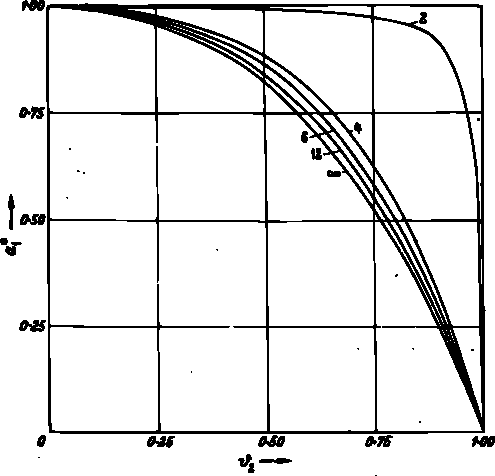
\includegraphics{../images/coordinate_number_dependence.pdf}
  \caption{无热溶液溶剂活度对溶质体积分数的曲线,不同$z$值的结果\cite{Tompa1956}。}
  \label{fig:coordinate_number_dependence}
\end{figure}

后世保持使用Flory--Huggins形式的惯例,有一定的合理之处。一般液体的平均配位数$z>6$。而数值计算结果表明无热溶液行为在$z>4$之后的差别很小(见图\ref{fig:coordinate_number_dependence})。因而混合熵部分采用Flory--Huggins形式有简洁方便的优势,至于混合焓部分,$q$与$r$的差别是否也总是可忽略?对于线形聚合物来说,
\[
  \frac{q}{r}=\left\{\begin{array}{ll}\left(z-1\right)/z,& r=2\\\left(z-2\right)/z,&r\to\infty\end{array}\right.
\]
因此考虑到实际$z<12$, 上面这样的比值不算特别接近1。可是,哪怕是逻辑自洽得到的式\eqref{eq:III.3_polymer_solution_mixing_gibbs_free_energy},也与大量实际体系的实验结果差别很大,主要来自仅考虑相邻作用势的假定。因此$q/r$是否足够近似于1的问题已经不重要。实践上常把式\eqref{eq:III.3_polymer_solution_mixing_gibbs_free_energy_flory_huggins}中的$\chi_{12}$视为一个唯象的可调参数,从而Flory--Huggins式成了至今大量采用的形式。
\end{document}